\chapter{Diseño e Implementación} % Main chapter title

\label{Chapter3} % Change X to a consecutive number; for referencing this chapter elsewhere, use \ref{ChapterX}
\definecolor{mygreen}{rgb}{0,0.6,0}
\definecolor{mygray}{rgb}{0.5,0.5,0.5}
\definecolor{mymauve}{rgb}{0.58,0,0.82}

\lstset{ %
  backgroundcolor=\color{white},   % choose the background color; you must add \usepackage{color} or \usepackage{xcolor}
  basicstyle=\footnotesize,        % the size of the fonts that are used for the code
  breakatwhitespace=false,         % sets if automatic breaks should only happen at whitespace
  breaklines=true,                 % sets automatic line breaking
  captionpos=b,                    % sets the caption-position to bottom
  commentstyle=\color{mygreen},    % comment style
  deletekeywords={...},            % if you want to delete keywords from the given language
  %escapeinside={\%*}{*)},          % if you want to add LaTeX within your code
  %extendedchars=true,              % lets you use non-ASCII characters; for 8-bits encodings only, does not work with UTF-8
  %frame=single,	                   % adds a frame around the code
  keepspaces=true,                 % keeps spaces in text, useful for keeping indentation of code (possibly needs columns=flexible)
  keywordstyle=\color{blue},       % keyword style
  language=[ANSI]C,					% the language of the code
  %otherkeywords={*,...},           % if you want to add more keywords to the set
  numbers=left,                    % where to put the line-numbers; possible values are (none, left, right)
  numbersep=5pt,                   % how far the line-numbers are from the code
  numberstyle=\tiny\color{mygray}, % the style that is used for the line-numbers
  rulecolor=\color{black},         % if not set, the frame-color may be changed on line-breaks within not-black text (e.g. comments (green here))
  showspaces=false,                % show spaces everywhere adding particular underscores; it overrides 'showstringspaces'
  showstringspaces=false,          % underline spaces within strings only
  showtabs=false,                  % show tabs within strings adding particular underscores
  stepnumber=1,                    % the step between two line-numbers. If it's 1, each line will be numbered
  stringstyle=\color{mymauve},     % string literal style
  tabsize=2,	                   % sets default tabsize to 2 spaces
  title=\lstname,                   % show the filename of files included with \lstinputlisting; also try caption instead of title
  morecomment=[s]{/*}{*/}%
}


%----------------------------------------------------------------------------------------
%	SECTION 1
%----------------------------------------------------------------------------------------
\section{Análisis del Hardware}

El prototipo se implemento sobre una EDU-CIAA en conjunto con un hardware de adaptación de las interfaces. Para ello se utilizaron los proyectos de código abierto kicad \footnote{\url{http://kicad-pcb.org/download/}} para los ponchos de la eduCIAA \footnote{\url{https://github.com/brengi/Ponchos}} para adaptar las entradas y salidas del conectores de expansión con los sensores y actuadores utilizados. 

\subsection{Sensores y actuadores}

\subsubsection{Esquemáticos del prototipo final}
% Aca van todo lo referido a consideraciones importantes sobre los esquematicos.
Para la adaptación de las interfaces con termocuplas y termistores se necesitaron para el primer caso de un circuito integrado compensador de juntura debido a la alinealidad en la respuesta de ese tipo de sensores. Para ello se eligió el (MAX31855KASA+) como una solución simplificadora. También existen soluciones de amplificadores multietapas con compensaciones que resultaban mas económicos, tal como el que se puede observar en la Figura \ref{fig:cirCompTermocupla} que se adapto para la termocupla usada en el prototipo.

\begin{figure}[h!]
	\centering
	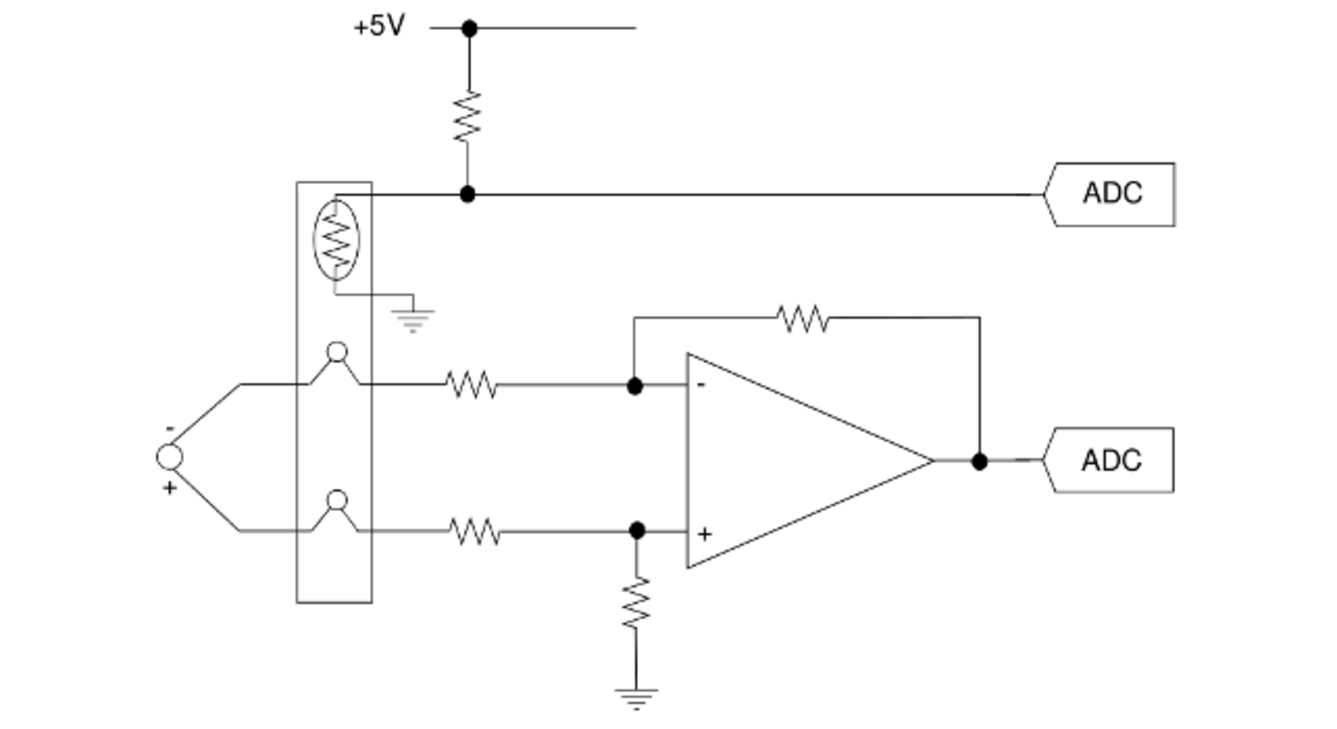
\includegraphics[width=.7\textwidth]{Figures/Cap_3/circuito_ampl_termocupla}
	\caption{Circuito simplificado de amplificación y compensación de termocuplas.} \protect\footnotemark
	\label{fig:cirCompTermocupla}
\end{figure}
\footnotetext{\url{http://ww1.microchip.com/downloads/en/AppNotes/00844a.pdf}}

Para el caso del termistor el circuito de adaptación fue mas simple debido a que señal obtenida es prácticamente lineal y solamente fue necesario amplificar a los niveles de trabajo de la entrada analógica del procesador. En la Figura XXXX se observa en tipo de circuito que se implementó.


\subsubsection{Renders del prototipo}

A continuación se muestran los renders de la placa de adaptación. En la Figuras \ref{fig:renderPonchoTOP} y \ref{fig:renderPonchoBOT} se ven las vistas del pcb prototipo propuesto a desarrollar para el sistema piloto. 

\begin{figure}[h!]
	\centering
	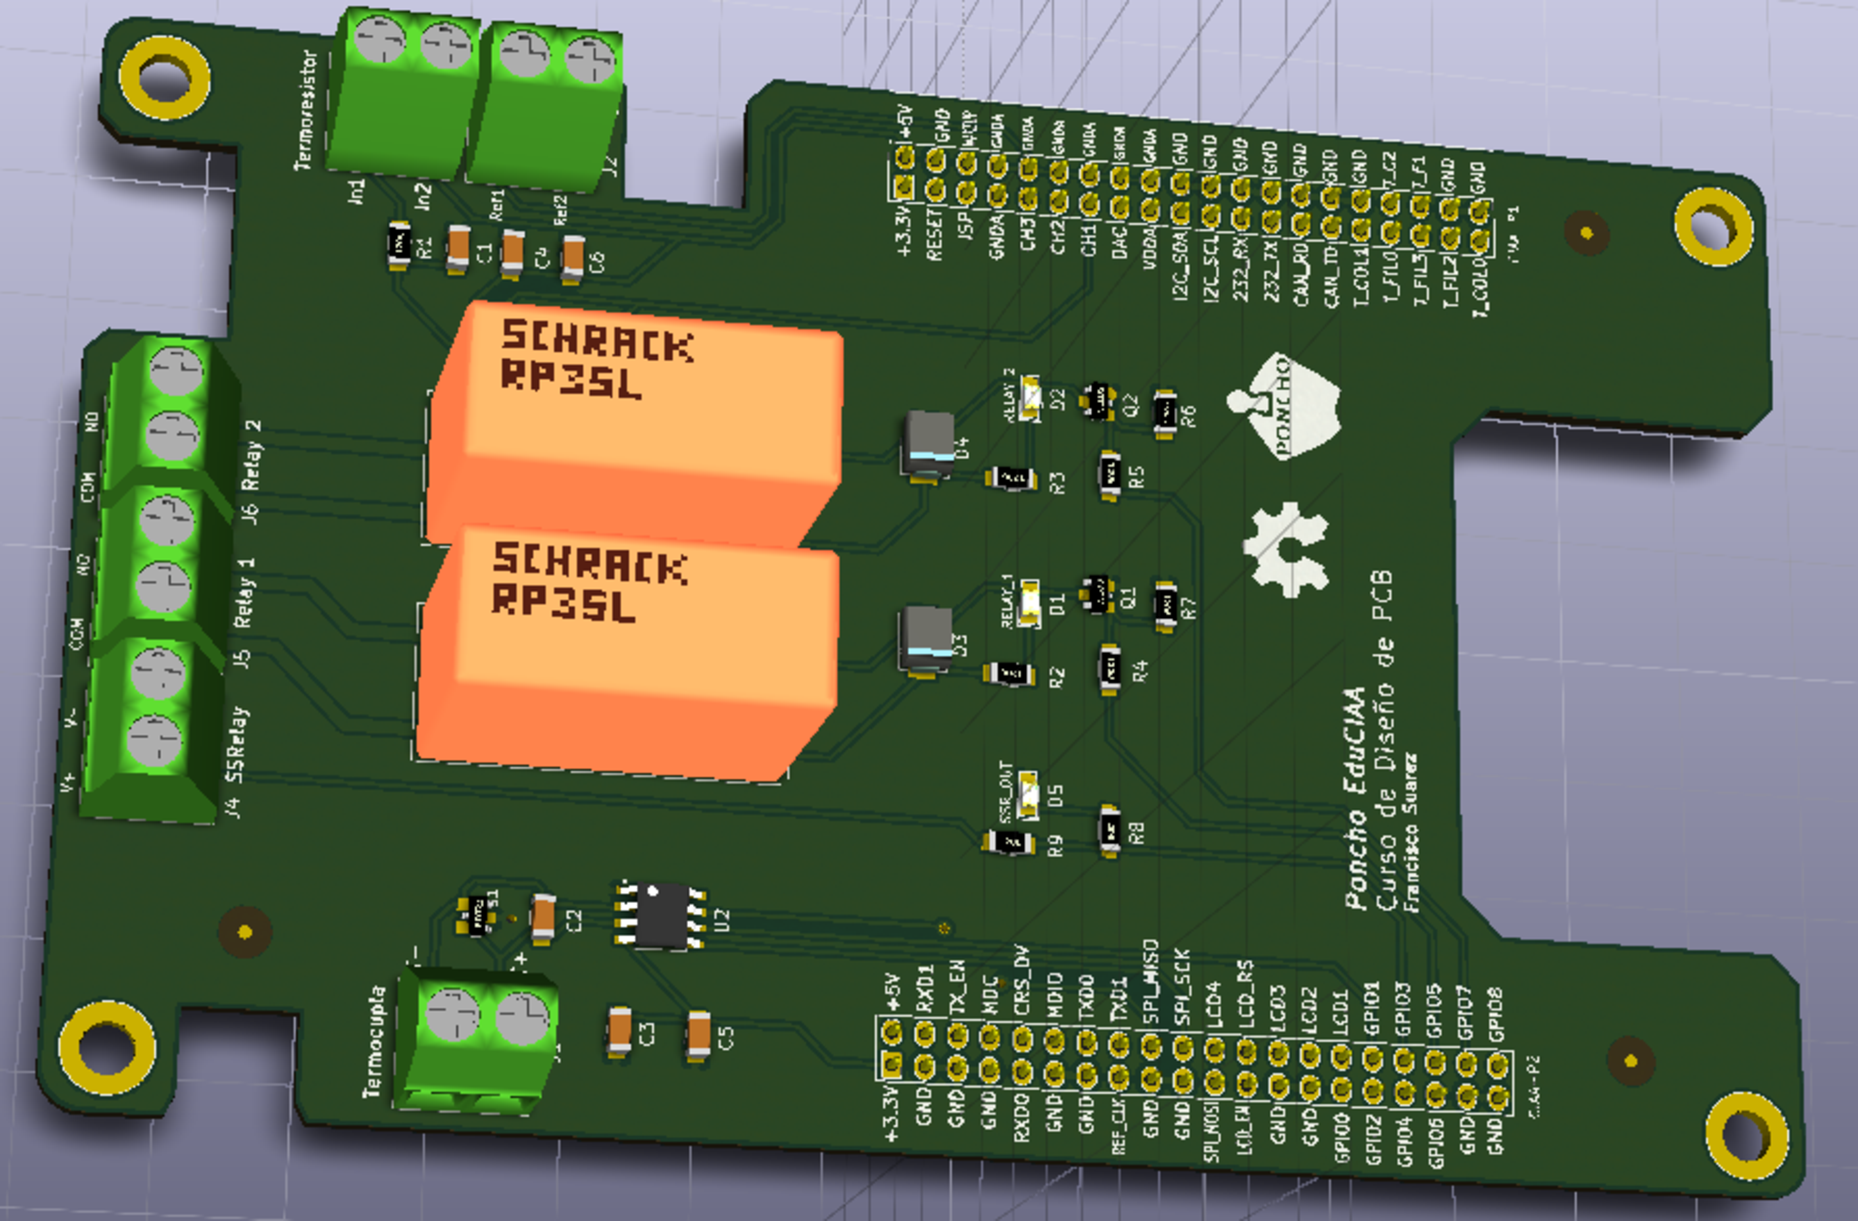
\includegraphics[width=.9\textwidth]{Figures/Cap_3/tempRelayPoncho_TOP}
	\caption{Render vista de arriba placa de interfaz.}
	\label{fig:renderPonchoTOP}
\end{figure}

\begin{figure}[h!]
	\centering
	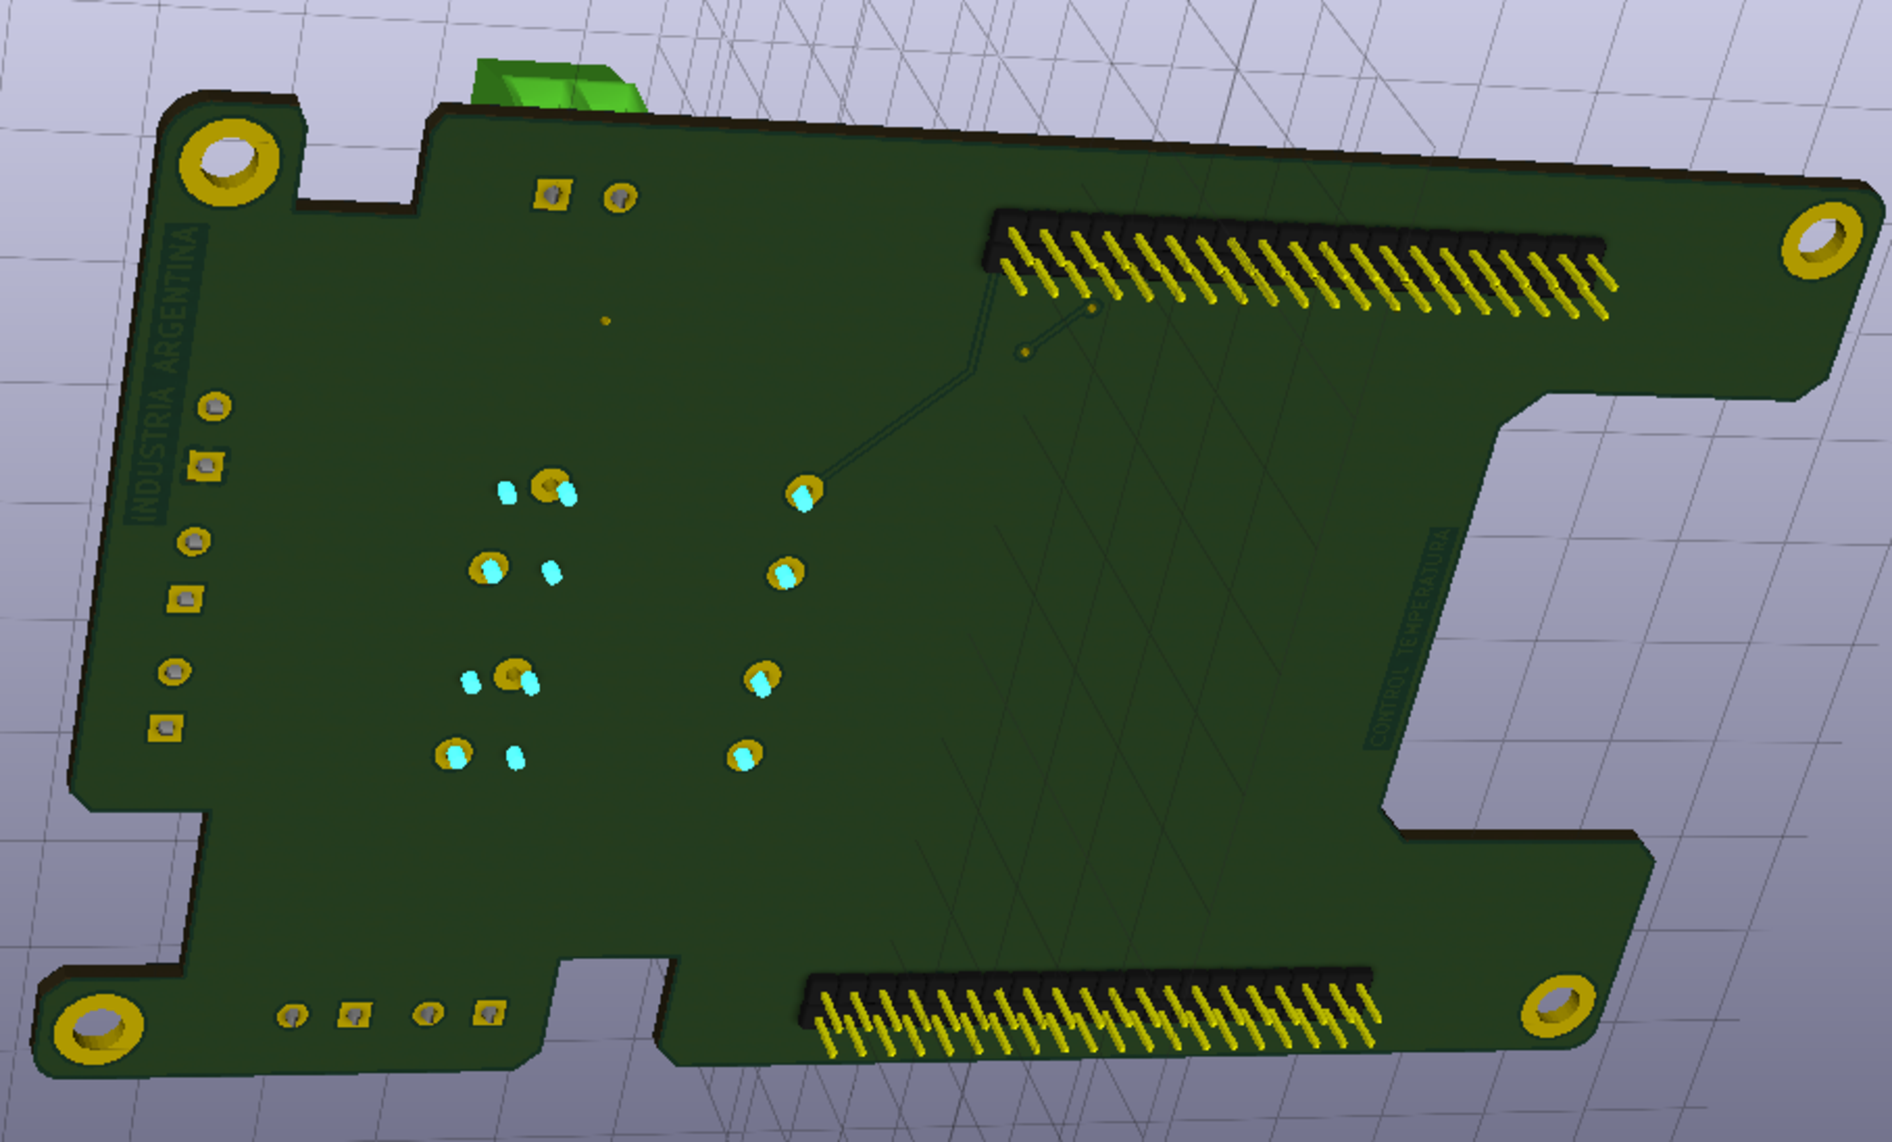
\includegraphics[width=.9\textwidth]{Figures/Cap_3/tempRelayPoncho_BOTTOM}
	\caption{Render vista de abajo de placa de interfaz.}
	\label{fig:renderPonchoBOT}
\end{figure}


%----------------------------------------------------------------------------------------
%	SECTION 2
%----------------------------------------------------------------------------------------
\section{Análisis del software}
 
La idea de esta sección es resaltar los problemas encontrados, los criterios utilizados y la justificación de las decisiones que se hayan tomado.

Se puede agregar código o pseudocódigo dentro de un entorno lstlisting con el siguiente código:

\begin{verbatim}
\begin{lstlisting}[caption= "un epígrafe descriptivo"]

	las líneas de código irían aquí...
	
\end{lstlisting}
\end{verbatim}


\subsection{Diseño del Firmware}
\subsection{Capas de abstracción}
% Agregar imagen diagrama con un el sistema prototipo.
\subsection{Arquitectura del Software}

Patrón de Arquitectura
Capas: 
\begin{enumerate}
	\item Abstracción HAL.
	\item Sistema operativo.
	\item Aplicación.
\end{enumerate}

Estas estructura permitió trabajar con mayor abstracción del hardware según la cual el problema se divide en partes y los esfuerzos se concentro en la capa de Aplicación que es la integra la lógica del sistema mientras que las demás administran los recursos del microprocesador. A continuación se ofrece una descripción mayor de cada una:
\begin{enumerate}
	\item Se utiliza para lograr una abstracción del hardware. Se piensa a futuro poder migrar el software de plataforma según lo requiera la tecnificación del momento. En este caso se utiliza la librería LPC OPEN.

	\item Se utiliza un sistema operativo de tiempo real a fin de hacer un mejor uso del procesador y los recursos disponibles para cada una de las tareas que la aplicación demande. En este caso se utiliza el FREE RTOS.

	\item La aplicación se basa en el patrón Control Ambiental en donde el sistema incluye sensores que proporcionan información sobre el entorno y los actuadores que pueden cambiarlo. Este patrón se aplicara utilizando en distintos módulos o tareas funcionales sobre el sistema operativo.
\end{enumerate}

Aplicación
La capa esta compuesta por los siguientes módulos:
a- Interfaz de usuario (ingreso de parámetros, uart, lcd, alarmas) 
b- Control de temperatura
c- Monitoreo de nivel
d- Monitoreo de conductividad
e- Monitoreo de energía
f- Control de tiempos

